\chapter[Introduction]{Introduction}
\label{cap:Intro}

\begin{Resumen}

This first chapter aims on giving the reader a panoramic overview of the problematic of study, raising consciousness on the work carried out through an introspective day-to-day approach PoV. Thus, the existing \nameref{sec:Intro:framework}\footnote{Projet HERGE was the teamwork in which my \ingles{stage} was framed, will be explained in detail in the section \ref{sec:Intro:thesis-purpose:HERGE}} is firstly stated, altogether with a \nameref{sec:intro:thesis-purpose:background} and a \nameref{sec:Intro:thesis-purpose} introduction, subsequently enriched in \hyperref[sec:Intro:Thesis-purpose:Outcomes]{management} and \hyperref[sec:Intro:Thesis-purpose-Budget]{financial} terms.

\end{Resumen}
\PartialToc
% ---------------------------------------------------------------------
% ---------------------------------------------------------------------

\bigskip
\lettrine[lines=2]{\textbf{A}}{}utomatization in any FoS, and neatly regarding image generation (AIG) has been markedly spread around multiples domains over the last decade, to the extend that it is presently being used for any kind of technology without us necessarily noticing out. Its threshold and applications vary from those most puristic ones, usually linked to the Artificial Intelligence (AI) branch (with a vast bibliography published on tackling human eye AIG recognition behaviour\footnote{The way in which humans systematically identify an object can be assessed and analyzed from the AIG's PoV} \cite{Eyevision}, annotation and description \cite{Automaticimageannotation,Automaticdescgeneration}, or semantic association \cite{Naturallanguage} in images generation processes), to those focused on a more pragmatic approach in Machine Learning (ML): developping genetic algorithms \cite{Genetic_algorithms}, image to text deep learning\footnote{Half-way between computer vision, natural language processing and AI, deep learning has been extensively used for sites, posts and, roughly, for any element of representation labeling} \cite{Deep_learning_image_to_text}, or software diagrams \cite{Software_diagrams} automatically.

Anyhow, a vast range of methodological algorithms for image generation of one-line diagrams have been successfully implemented in recent years \cite{Distribution-feeder,standard-based-SLD-AG,AlgoAIG}. Such being the case of our object of study, its practical use strictly based on a corporate database source, deeply suggested an integrated data treatment process. Hence the interest of \href{https://www.safe.com/how-it-works/}{Feature Manipulation Engine (FME)} usage, a powerful tool fed on web-sources, application and any kind of data roughly speaking, which, via its conglomeration and the enhancement on logically-linked image displaying thanks to \href{http://www.esri.com/}{Environmental Systems Research Institute (ESRI)} - \nameref{sec:approach:software:ArcGIS} technologies, has finally resulted on a rigorous, edge-cutting, still intuitive corporate tool. 

With this aim, a methodogical process for automatic Rte's network diagram representation is proposed on this work. Remarkably, the latter being completely adaptable to corporate patrimonial databases while being performed on departmental  tools, as those previously stated. 
% ---------------------------------------------------------------------
\section{Framework}
\label{sec:Intro:framework}

My final-degree internship project has been pursued as part of HERGE, which governed by GAME - \ingles{Gestion Anticipée et Maitrise de l'Exploitation} - team, constitutes all at once an important part of DPOSE - \textit{Département Programmes et Outiles du Système Electrique} - dept. All those, contained in the DSIT - \ingles{Direction Systèmes d'Information et Télecom} - dept., constitute the latent force of Rte - \ingles{Réseau Transport d'Electricité}'s technical solutions development. 

Two tutors (\texttt{Jean-Etienne Lemaire} in a first 3-months time-lap, and \texttt{Philippe Rapin} in the coming three) have encompassed my activity in the context of HERGE, with the constant assistance of \texttt{Heng Ngeth} in technical and bureaucratical matters. 
Henceforth, all these elements will be concreted in detail from a macroscopic to a technically tangible horizon going over the stages from the \hyperref[sec:Intro:Rte]{entreprise} scope, to the \hyperref[sec:Intro:thesis-purpose:HERGE]{project in question's}: 


\subsection{Rte}
\label{sec:Intro:Rte}

Rte is born in 2000 as a result of \href{https://eur-lex.europa.eu/eli/dir/1996/92/oj}{\texttt{European Directive No. 96/92/EC of December 1996}} aiming to completely keep generation and transmission national companies independent. Four years later, Rte's activities completely unbundled EdF's - \textit{Electricité de France} - and therefore their divestiture finally becomes a reality, granting its trademark rights from them on.

The sole Transmission System Operator (TSO) in metropolitan and continental France plays a strategic role that goes way beyond the implicit meaning of the term "power transmission" gatewaying geneartors, industirial consumers MV distributors, rail companies and market traders  activity.

\begin{figure}[h!]
    \centering
    \parbox[t]{0.6\textwidth}{
    {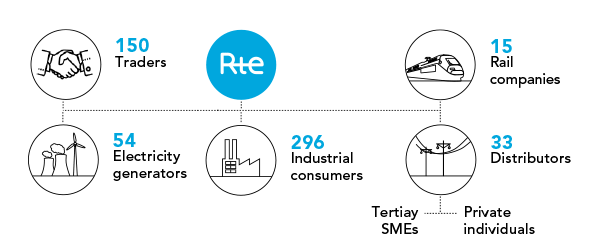
\includegraphics[width=0.6\textwidth]{0.figuras/clients.png}}
    \captionof{figure}{Rte clients portfolio.}}
    \label{fig:Rte-portfolio}
\end{figure}

Within a strictly-regulated framework supplying grid access in completely fair competition, as overseen by the Energy Regulatory Commission (CRE), Rte balances its grid round-the-clock, while broadening its ressources of tomorrow in order to \textit{"ensure security of supply and sustainable electricity system operation, to guarantee the same quality of service for everybody, to continually improve our services, and to contribute to the economic development of the territories"} (citing expressly from the corporate webpage).

With nearly 105,000 km of lines, RTE has eversince canalized the national and international financial activity through the biggest grid in whole Europe: 46.2 \% of which extra-high voltaged lines (400 and 225 kV\footnote{Regional sub-transmission is performed at 150, 90 and 63 kV}), which rout annually about 495 TWh\footnote{Annual energy transit flow remains virtually steady over the last years \cite{IEC-normative}.} all over the hexagon and \href[https://www.rte-france.com/sites/default/files/2015_05_20_flow_based_brochure.pdf]{beyond}, where reaching 112 TWh thanks to 60 cross-border connections with neighbouring countries.

\begin{figure}[ht]
    \centering
    \parbox[t]{0.475\textwidth}{
    \centering
    {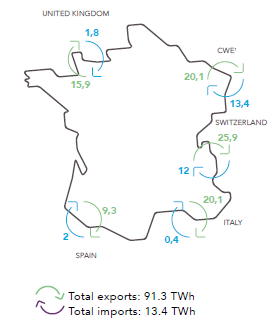
\includegraphics[width=0.475\textwidth]{0.figuras/exports-imports.png}}
    \captionof{figure}{International exports-imports flux.}
    \label{fig:Rte-portfolio}
    }
    \hfill
    \parbox[t]{0.475\textwidth}{
    \centering
    {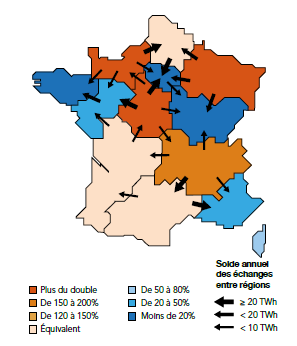
\includegraphics[width=0.475\textwidth]{0.figuras/prod-consumption-national.png}}
    \captionof{figure}{National flux exchanges between regions in 2015.}
    \label{fig:National-exchangues}
    }
\end{figure}



Its employees continuous training program empowers its mainstay: e.g. the versatile knowledge and visibility of its high-skilled 8,279 employees-officials workforce, responsibles of the exploitaton and maintenance of 1,231 transformers, 2,710 substations and 3,504 delivery points, whose rate of burying between 2014 and 2015 reached a 97 \%.

RTE, with an actual turnover of €4,126 million in 2007, and yielding a profit of €466 million\footnote{Both up slightly from previous year, which RTE attributed to increases in network access payments and interconnector capacity auctions revenues.}, has constantly endeavoured to offer its customers safe, economic and clean access to electrical power. There is no shortage of projects: extension of market coupling to Southern European countries, installation of smart substations, using drones to maintain infrastructures...
%REVISAR ULTIMO PARRAFO

%ANADIR IMAGNES GRAFICOS LOGO??	

\subsection{DPOSE}
\label{subsec:Intro:thesis-purpose:DPOSE}

Hierarchical continent of HERGE, DPOSE conforms the Rte's tool development dept., as its literally labelling translation\footnote{Electric Systems tools \& software Dept.} stands for. And its actual functionalities do not differ much from that: formed by a team of engineers highly trained in software development and abstract thinking, HERGE feeds Rte with a vast range of software conception, development and, finally, industrial production launch. Branched in 5 big subsections, and grouping about 100 employees, they are as follows:

%HABLAR CON GUILLAUME PARA CADA UNA DE ESTAS RAMAS

%FORMATO DE LA TABLA QUE TENIA ANTES
%{
%\setlength{\extrawaheight}{2ex}

%\begin{longtable}{@{} >{\ttfamily}p{0.1\textwidth} @{\hspace{0.01\textwidth}} p{0.85\textwidth} @{}}
\begin{description}


\item{\textbf{GAME -} \ingles{Logiciels DV} - Software DV.} GAME frames the whole dept.'s activity, by proposing technical solutions in terms of applications and human-machine interface (HMI) \ingles{Mise en production} (MEP), that is, projects channelling from their conception to the final industrialization launching.
 \\

\item{\textbf{OSCAR (\ingles{Outil de Saisie des Contrats d'Accès au Réseau}) - }\ingles{Management en temps réel} - Real-time management.}   It is responsible of ensuring project continuity exploitation in the real time, making solutions animated by other departments physically possible and therefore to make them become a reality. Neatly, it manages the different clients' portfolio automatic access to the electrical network.\\

\item{\textbf{SID (\ingles{Système d'Information Décisionnel}) - }\ingles{Héberger} - Host.} In charge of the inter-applications info management, by fire-walling its flow through telecommuted devices.\\

\item{\textbf{StanWay - }\ingles{Conduire} - Carry}. The future communications tool. It is destined to replace SRC and SNC actual system in all the exploitation centres.\\

\item{\textbf{STEP (\ingles{Systéme Téleconduite Et Passarelle}) - }\ingles{Configurer} - Configure.} Data management tool. It encompasses the different \texttt{steps} information takes.\\

\end{description}
%\end{longtable}

\begin{figure}[h!]
    \centering
    \parbox[t]{0.6\textwidth}{
    {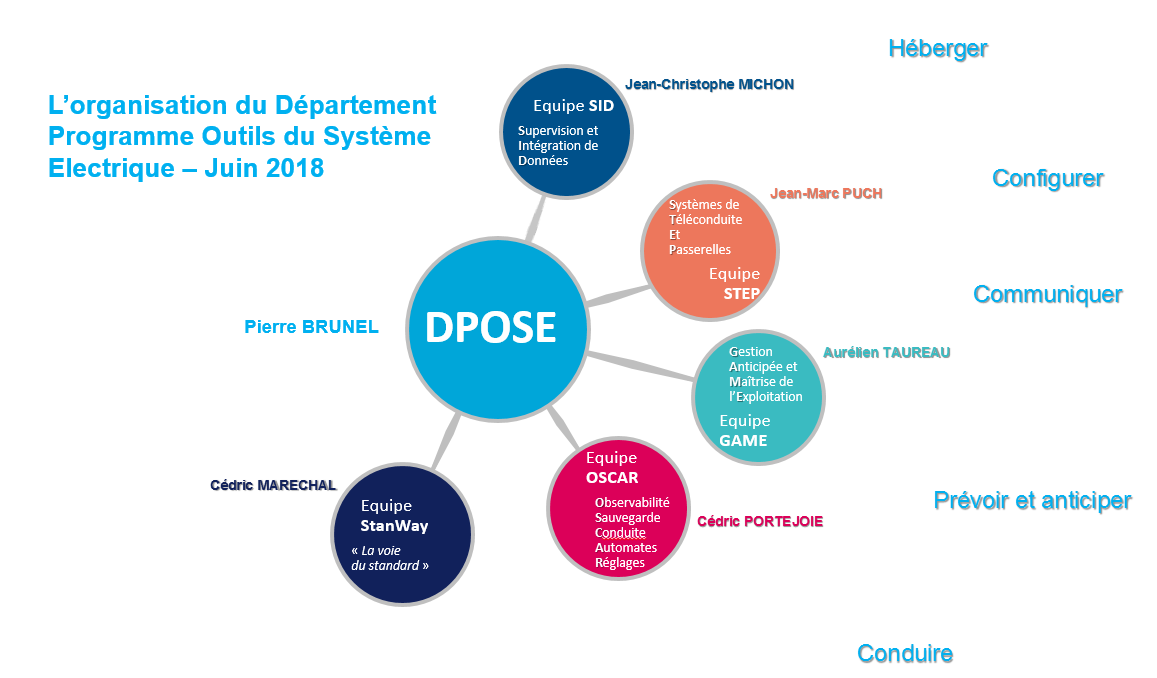
\includegraphics[width=0.6\textwidth]{0.figuras/DPOSE.png}}
    \captionof{figure}{Projects hierarchical interdependences within DPOSE.}}
    \label{fig:DPOSE}
\end{figure}

\subsection{HERGE}
\label{sec:Intro:thesis-purpose:HERGE}

Framed around a 5-person team and leaded by my tutor Jean-Etienne Lemaire, whose functions were retaken in early August by Philippe Rapin, HERGE consists of a mulitidsciplinary high-formed team of engineers, aimed to create an intutive and interactive interface of the french HV\footnote{Henceforth we will consider \texttt{High Voltage, } for tensions from 63 to 400 kV, commonly designed as the \texttt{Transport phase}.} and eventually MV\footnote{We will consider \texttt{Medium Voltage}, for tensions from 4 to 63 kV, commonly designed as the \texttt{Distribution phase}} electrical network, discredited in 7 regional zones represenation, plus a national one.
Framing the project in the tools-developping section for Operation Management anticipation (DPOSE), it consists of an ambitious project focused on three key activities:
\begin{itemize}
    \item \textbf{Represent} graphically the network and its subconstituents unequivocally and perennially over time.
    \item\textbf{Provide} all the corporate SRC and SNC users with a unique and lisible network layout representation, enabling its perfect contextualization.
    \item \textbf{Normalize} network representation for the Exploitation Dept. at any time horizon.
\end{itemize}

\begin{figure}[h]
    \centering
    \parbox[t]{1\textwidth}{
    \href{https://herge-portal.rte-france.com/arcgis/apps/webappviewer/index.html?id=84a7af442f014844bd95939ce3c0067a}{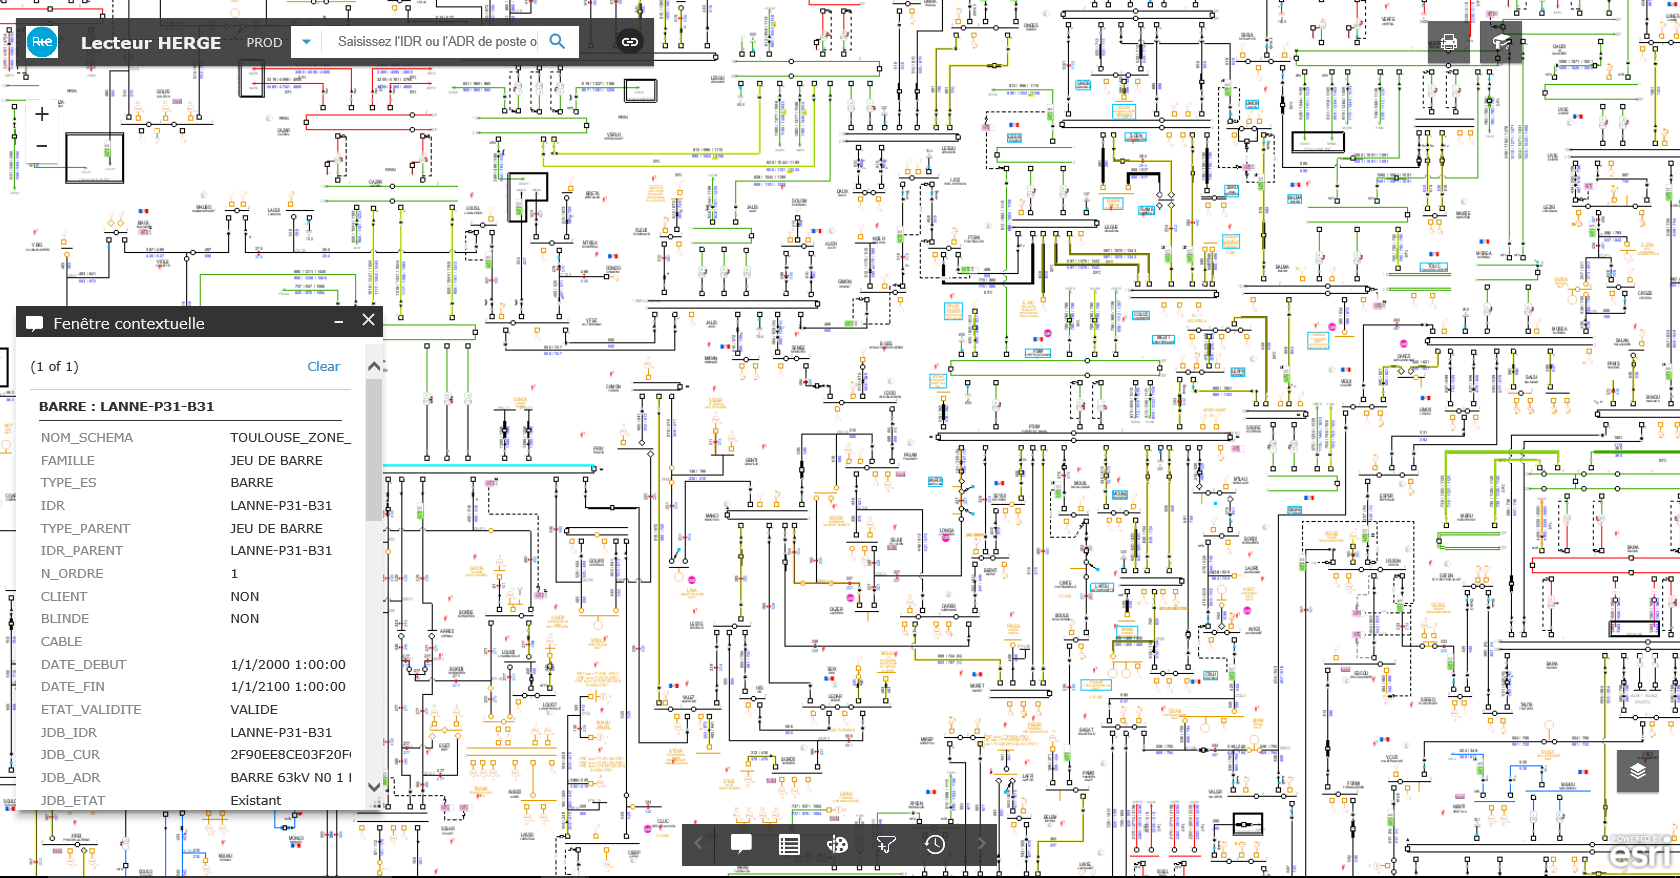
\includegraphics[width=1\textwidth]{0.figuras/HERGE_interface.png}}
    \captionof{figure}{HERGE interface layout. Click on the image to acces RTE's electrical diagram layout interface}}
    \label{fig:herge}
\end{figure}

%QUITAR IMAGEN ORGANIZACION OPERATIVA DSIT

%\begin{figure}[h]
   % \centering
    %\parbox[t]{1\textwidth}{
    %\href{}{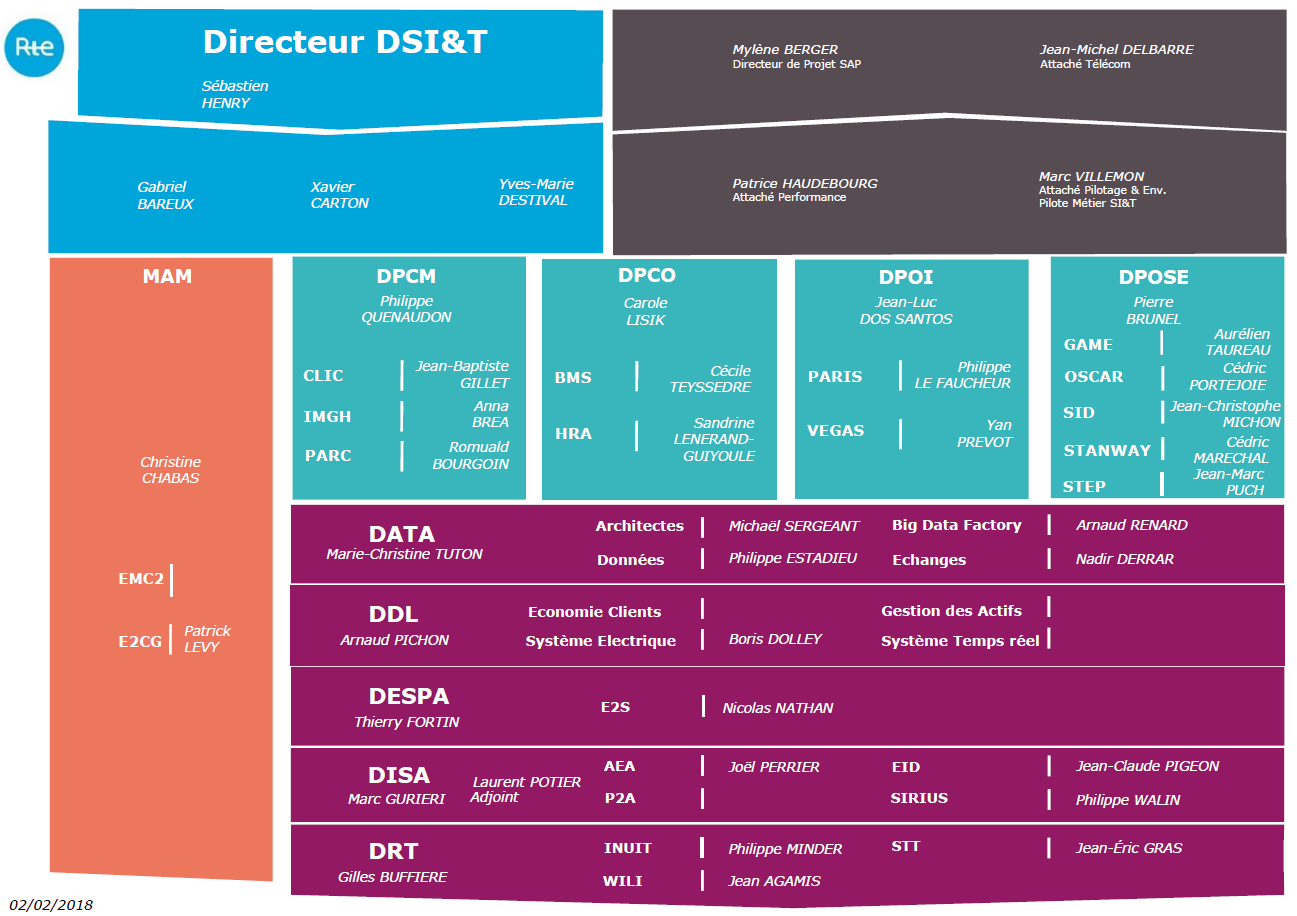
\includegraphics[width=1\textwidth]{0.figuras/DSIT_organization_chart.png}}
    %\captionof{figure}{DSIT organizational chart. HERGE is contained in GAME Dept., under the lead of Aurélien Taureau.}}
    %\label{fig:dsit}
%\end{figure}

%UNIR CADA UNA DE LAS ZONAS A UN PLANO EN ANEXOS???

HERGE is therefore responsible of displaying the electric diagram layout for the 7 zones (\ingles{CNES Quart, Lille, Lyon, Marseille, Nancy, Nantes, SQY Po and Toulouse}) where SRC has been discretised. Henceforward, HERGE will enrich the former electric diagram with a voltage colour coding, plus  elements ordering control possibilities, thus giving birth to \nameref{cap:AIG} of Herge. 

As defined in its corporate culture, RTE's employees are not expected to remain in a certain post for more than 4 year. This fact boosts the common collective feeling and enlarges the competences field of all workers. Furthermore, it turns  documentation into a vital tool for ensuring continuity of the projects, which frequently exceed its members' stay. 

Additionally, HERGE's specifications expect it to become a real-time version, and may have very interesting potential application in the foreseeable future. Specifically, it seeks to provide the dispatcher with a tactile interface, intended to make its layout interpretation easier, clearer and therefore much more efficient. Therefore a first step towards HERGE's amortization has been bureaucratically already materialized. Not only this fonctionallity will embrace its old functions, but will also step forward as a referent for other projects feeding, with consequent inter-projects iterations for everyone's tender specifications meeting. Neatly, regarding StanWay's influence, conversations have already begun and exchanges between projects are more common, and more appropiate.

\subsubsection{Corporate framework}
\label{subsubsec:Intro:thesis-purpose:Framework:corporate-framework}
Framed in a multidimensional environment, the present project impacted and was impacted by a wide spectrum of factors of all kinds, which are explained with detail in the following.
The usage of independent layouts, even throughout a same enterprise is widely spread among Rte's non-concomitant projects. Each of them are displayed according to different basis, and it's under this non-uniqueness representation model that underlie many of the daily problems in a daily HERGE's employee day-to-day life. It is on this basis that several inter-departmental  meetings were hold between members of the teams STANWAY and APOGEE in order to enrich mutual knowledge and approaching of a mutual problem, and standardize thereafter an unique representation criteria, noting projects' aims diverged considerably seldom.

In addition, HERGE responsibilities and application diverge from a wide range of projets and departments, and therein resides the fundamental difficulty of the problem. Hereafter, a full list of the potential daily HERGE users is displayed. 

\begin{itemize}
    \item\textbf{Operation Management Dept.-} \ingles{Service Conduite} - 293 employees: in charge of the weekly updating, corresponding to the instant t.
    
    \item\textbf{Planning Management Dept. -} \ingles{Service Planification} - 151 employees: in charge of the network evolution. Using network schemes for incoming activities planning.
    
    \item\textbf{Strategy Dept. -} \ingles{Service Strategy} - 99 employees.
    
    \item\textbf{Performance Dept. -} \ingles{Service Performance} - 58 employees.
    
    \item\textbf{Maintenance Dept.}
    
    \item\textbf{Research \& Developpement Dept. -} \ingles{Développement et Ingénierie}.
    
    
\end{itemize}


All those stakeholders, potentially impacted by the numerous approach changes undertaken, constitute a big part of the enterprise activities. Whatsoever, by the moment of my arrival, Herge's approach was completely alien to StanWay's, hoping it is not that much by the moment I leave the project, the following actions have been taken. 

In particular, all the stakeholders were contacted and put together in order to overcome with the optimal solution for the inital purpose of alleviating this objectives' misalignment, leading to a considerable consciousness-raising of the bureaucratic side within such a multilateral-concerned project. Decisions were taken with mutual consent and efforts were mainstreamed in the pursuit of every part's best, contributing all this to ramp up the intern's skill and integration within the work-group.

\begin{description}

	\item\textbf{Herge}: DPOSE-branched subsection, it aims on an interactive web interface realization. Further information has been provided in the section \ref{sec:Intro:thesis-purpose:HERGE}, with an aim in deeper \ingles{raison d'être} explanation and specific roles detailing.

	\item\textbf{StanWay}: also DPOSE-branched, it is a project in charge of the new corporative SCADA deploiement. SCADA (Supervision Control And Data Acquisition) is a \textit{"control system architercture that uses computers, networked data communications and graphical user interfaces for high-level process supervisory management"} (Wikipedia).
	
	\item\textbf{Itesla}:  Research and Development (R\&D) Dept. - branched, independent from DPOSE's continent, e.g. DSIT (\ingles{Direction des Systèmes d'Ingénierie et Télecom)}, and in charge of the former SCADA deployment, it puts together a various and numerous set of teams, working altogether for the RTE of tomorrow.
	
	\item\textbf{Convergence}: Moreover, than a departement, it represents a deeply-shared tool that makes the reformating and interexchangue of the multiple format types possible. It boosts therfore the continuity of all kind of problems, even if their approaches may diverge considerably at first sight. 
	
	\item\textbf{Apogee}: ITESLA-branched, they display real-time breaker changes due to operator decision and/or unexpected events. Their Java-sourced approach is consistently different, but the target and delivrables stay pretty close to HERGE's, and relatively interchangable via CONVERGENCE's archive reformatting. Indeed, they delivred .iidm files as their doc outcome.
	
\end{description}

Anyway, Rte departamental structure consitute a knowledge network  Multidimensional knowledge sharing between all these projects has been vital for profitable evolutions in a participatory way, thanks to Rte's proactive philosophy underlying.

\subsubsection{Educational framework}
\label{subsubsec:Intro:Thesis-purpose:Framework:Educational-framework}

In educational terms, this documents constitutes at once several independent livrables, framed all them in the pursuit of my studies. It will firstly be my Master in Industrial Engineering's Thesis, as \ingles{Trabajo Final de Grado}\footnote{Master's Thesis equivalent in Spanish educational regulatory framework} of a 4-plus-2 years Bachelor's \& Master's degree program in the \ingles{Universidad Politécnica de Valencia}. At the same time, this document represents the \ingles{Travail de Fin d'Etudes} of \ingles{Ecole Centrale Marseille}'s studies i.e. a 3-year academical course final thesis, as a part of a Double Master simultaneously there pursued.
All at once, it gathers all the procedure undertaken during a 6-month internship as \ingles{Stage de Fin d'Eudues}, for which this documents constitutes its \ingles{Rapport de stage}\footnote{End of Studies internship's report in French educational regulatory framework.}.

%Tambi�n encontrar�s un archivo denominado `\texttt{preambulo.tex}', donde hemos incluido algunas configuraciones y macros personalizables. Puedes aprovechar este archivo para cargar los paquetes adicionales que utilices en tu publicaci�n.

% ---------------------------------------------------------------------
\section{Thesis purpose}
\label{sec:Intro:thesis-purpose}

The final goal of this Master Thesis's lies on the automatizing of Rte's electrical layout diagram, as a part of the HERGE projet. The team had already an interface prototype running, completely functional and performing, but in which elements dispositions had been previously handmade in AutoCAD by an architect, and no-automatizing was displayed, apart from certain elements labeling.

Numerous stakeholders were affected and interested by this corporate challenge and that influenced considerably the project scope and so did it its approaching too. It was finally those stakeholders who both will afterwards get use of the app outcome and had financed its implementation.

% ---------------------------------------------------------------------

\subsection{Background and \ingles{état de l'art}}
\label{sec:intro:thesis-purpose:background}

Nowadays, the major issue before research and energy industry is the mounting uncertainty that complicates financial viability of the major investments required for the development of edge-cutting technologies and innovative projects. IoT\footnote{Internet of things, refers to the interconnection of multiple devices to transfer autonomously all kind of data, aiming to shorten physical and digital worlds gaps.}: Block-chains, miners, Artificial Intelligence, 3D-printing are some of the edge-cutting technologies promoting this sudden turnarounds in the last decade, which are "likely to be more dramatic than those undertaken during the last century altogether"\footnote{citing explicitly the book 'How Customer Behaviour and Technology Will Change the Future of Financial Services'.}. Enterprises seem to be increasingly concerned on this matter, and are markedly reshaping their business models and working methods. Nevertheless, the emergence of multiple business domains and the big reticence has boosted startups spread-up.   
Rte, well aware of this reality, is turning its sight into edge-cutting, modern projects, such as Apogee, Stanway, Itesla, etc. Herge is indeed one of those potentially high-impact projects in an environment where lot of potential profit underlies, as shows the wide literature and software deployment in the FoS of any nature of LD's AIG, which traditionally hand-desingned. Worth of special mention is \nameref{sec:Diagram:CIMDesk} software, used by Stanway, and which served us for symptomatic processes correlation. 

\begin{figure}[ht]
    \centering
    \parbox[t]{0.475\textwidth}{
    \centering
    {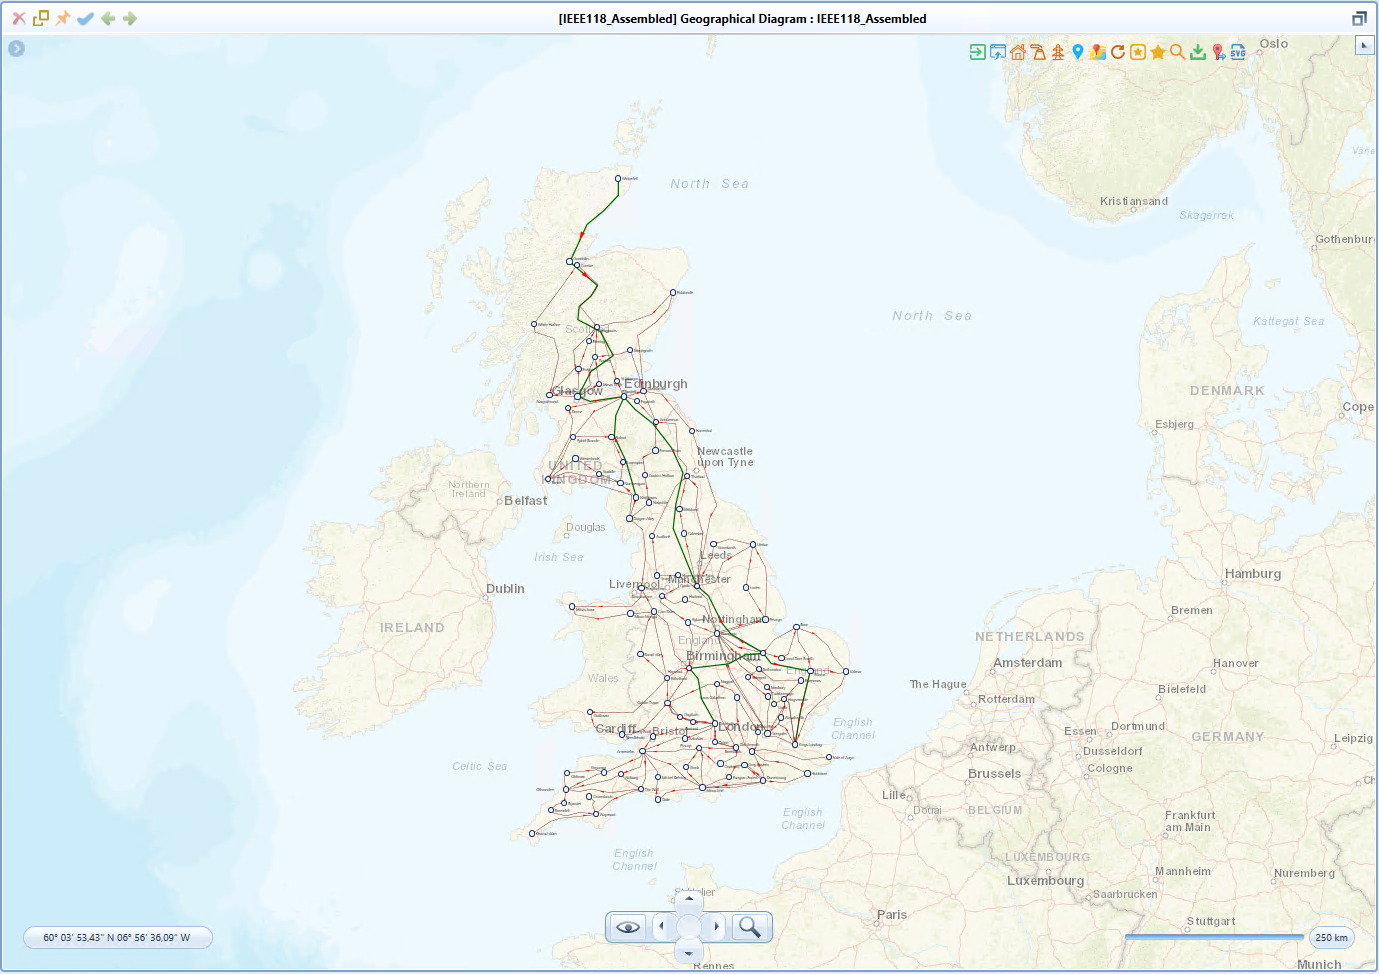
\includegraphics[width=0.475\textwidth]{0.figuras/CIMdesk_england_chart.png}}
    \captionof{figure}{England electric network flux chart displayed with CIM Desk.}
    \label{fig:CIMDesk}
    }
    \hfill
    \parbox[t]{0.475\textwidth}{
    \centering
    {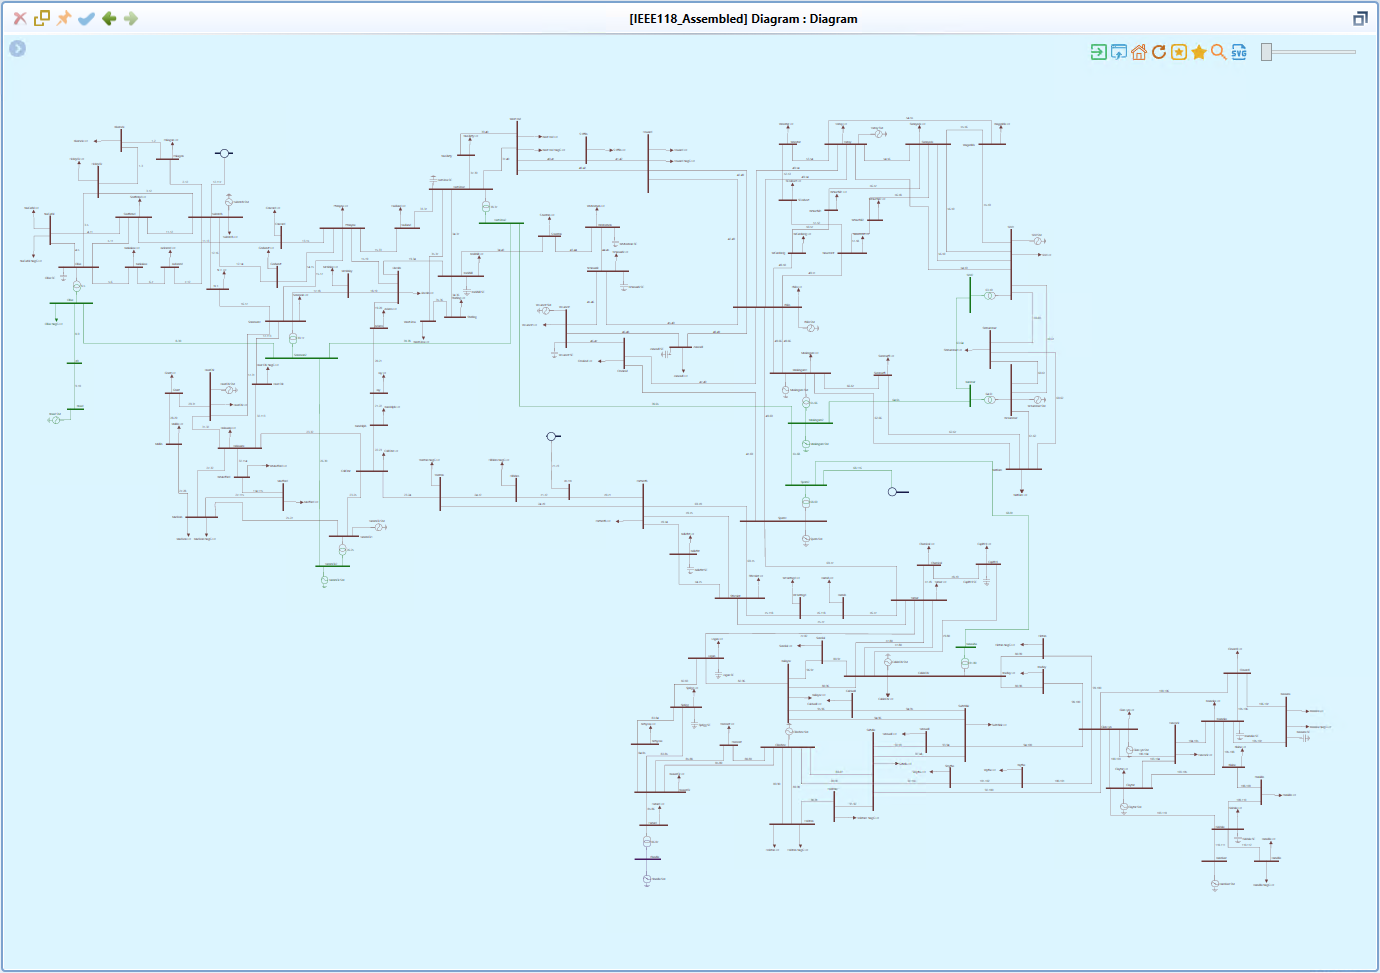
\includegraphics[width=0.475\textwidth]{0.figuras/CIMdesk_england_network_electrical_chart.png}}
    \captionof{figure}{England electric network diagram drawn from its flux chart interpretation with CIM desk.}
    \label{fig:CIMDeskdiagram}
    }
\end{figure}

A vast range of design software exists onto Computer Aided-Design (CAD) of electrical LDs: \textit{See Electrical, DesingSpark Electrical, Bentley's Promis-E, Eplan Electric} or just the \textit{AutoCAD Electrical Toolset} are CAD-based tools that enabled certain automatizing in electrical block components introduction, which finally are to be hand designed by an architect. Thus their automatizing from databases patrimonial remaining certainly unexplored, the necessity of CIM Diagram Layout (CDL) interfaces for streamlining the whole processes is therefore sufficiently substantiated.

Consequently, an skill improvement in XML, RDF and other database formats understanding and contextualizing has been carried out, as seen \hyperref[fig:UMLprofile]{in the following UML class diagram}. To achieve the target goal of network architecture automatizing, deep database usage seems to be the best technically feasible solution in the short term \cite{Automaticdescgeneration, CIMIEE, CIMDistribution}. In addition, and  profiting the corporate patrimony and extensive knowledge of several Rte's employees \cite{specif_detaillees_GAI, IEC-normative, Infos_GAI} of the state of art among the principle european and international distribution companies, a standardized database treatment process was pursuit.

\begin{figure}[h]
    \centering
    \parbox[t]{0.8\textwidth}{
    \centering
    {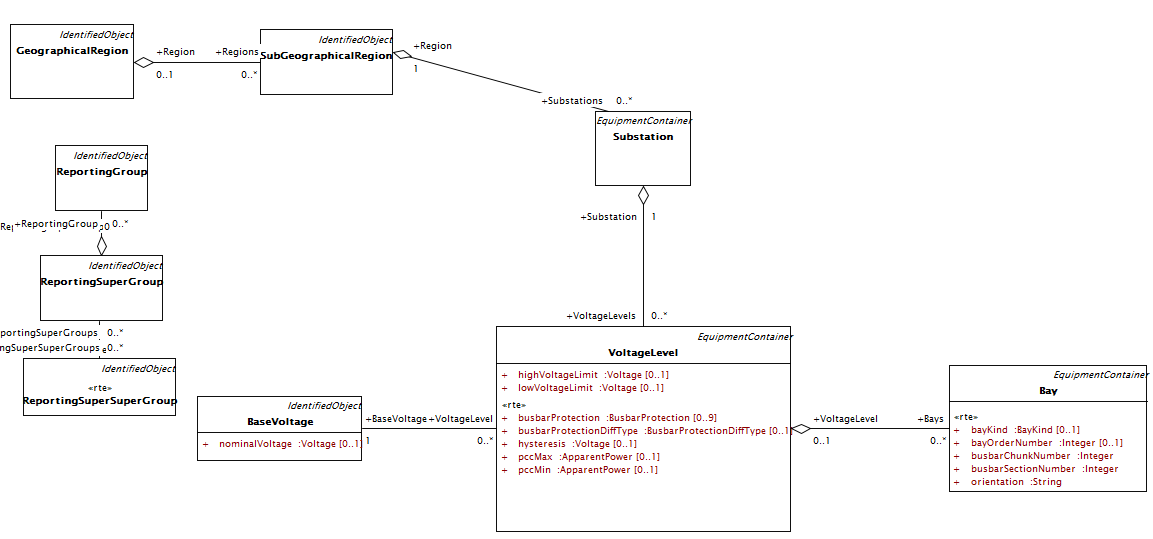
\includegraphics[width=0.8\textwidth]{0.figuras/UML_RTE_geographical_region.png}}
    \caption{UML profile of the substation level dependencies.}
    \label{fig:UMLprofile}}
\end{figure}

Indeed, certain steps have been already taken ahead troughout interesting development studies on the topic, undertaken in SouthKorean \cite{standard-based-SLD-AG} and Indian \cite{Distribution-feeder} research centers. Being the majority of those projects code-oriented \cite{Eyevision, CIMjava}, that is, their deployment sustaining in a low-level language coding implementation, Herge diverges from this approach and comes up with a more intuitive, user-oriented approach. Thus, basically based on the use of \nameref{sec:approach:software:FME}, and relying on corporate patrimonial database refreshment, this software is intended to turn the way AIG of diagram layout have traditionally been designed upside down. 

%%\begin{figure}[h]
    %\centering
    %\parbox[t]{0.8\textwidth}{
    %\centering
    %{\includegraphics[width=0.8\textwidth]{}}
  %%  \captionof{figure}{UML profile of the substation level dependencies.}}
%%    \label{fig:UML_profile}
%%\end{figure}

Some avenues of recourse that could enrich the FME post-treatment have been explored and assessed, mainly \nameref{sec:approach:software:ArcGIS}-linked for post position management for the purpose of a better space usage and interconnection network optimization. Those exploitation routes are deduced from the implementation \nameref{subsub:AIG:SLV:graph_theory}, \nameref{subsub:AIG:SLV:graph_theory:meta_algorithms}, \nameref{subsub:AIG:SLV:Voronoi} or Multidimensional Scaling (\nameref{subsub:AIG:SLV:MDS}) to the problematic of study. All of them are discussed in detail in section \ref{sub:AIG:SLV:theoretical background}.

%INSPIRARSE EN EL ARTICULO SOBRE BOCKCHAIN DE IGNACIO MADRID ENCONTRADO EN LA REVISTA SMART GRIDS INFO QUE HE GUARDADO EN MARCADORES

% ---------------------------------------------------------------------
\subsection{Project approach}
\label{sec:introduction:thesis-purpose:project-approach}

Constituting the graphical interface for the most part of Rte's on-field business users, an important flux of financial actives depend on Herge's fate, which makes it a substantially constrained project in terms of users necessities. They are the ones who grab the major part of the negotiating power and therefore who encompass the trail of the project.

Consequently, the results of the displayed methodology shall remain certainly close to the actuals, and changes may be considerably evident, flexible and easily apprehensible. This incertitude reigning all the project long has deeply impacted its approach and methodology, always on the pursuit of flexibility by means of modularity and adaptability possibilities in connection to the future additional steps Herge could take, yet as all its impacted partners.

Apart from the technical approach, a managerial PoV was assessed all along the project, as it remained absolutely non static and deeply impacted by the approach during certain evolution phases. For this reason and overall on the skill ramp-up periods, several meeting were held with the automatic network representation mainstream corporate voices on the matter for a proper state of art drafting, and the different technical solutions to address sketching.

In this purpose, \hyperref[subsub:introduction:thesis-purpose:project-approach:parties]{several ateliers and meetings} have been arranged specially on the ferirst stage of the internship for boosting a correct sill ramp up altogether with a project contuxtualization.  To confront the incertitude coming from a vast range of inputs, \hyperref[subsub:introduction:thesis-purpose:risk-assessement]{a risk matrix }has been performed at the first stages of the project. It has been nevertheless systematically completed in the face of changes found progressively, and notably after identifying other projects adhesions.


\subsubsection{Concerned parties}
\label{subsub:introduction:thesis-purpose:project-approach:parties}

In this line, numerous stakeholders have been confronted through the project contextualization. Their roles and importance divergence between them, and their interdependence with Herge impacts its actions and viceversa.

The main projets that were contextually confronted to Herge are as follows:
\begin{description}
    \item[- StanWay:]
    One of the biggest projects in Rte at the moment. 35M€-budgeted, it aims to create a huge data exchanging platform, for the different levels of corporate data acquisiton, and, regarding us, for SCADA structure layout deployment.
    \item[- Apogee:]
    Inside the DDL department, it consists on an coding platform, striving for homologous purpose to StanWay's. I.e, energy real-time flux management
    
\end{description}

\subsubsubsection{StanWay}
\label{sec:approach:project-approach:parties:stanway}

The information flux was continuous and considerable between both projects, whereas their approaches and objectives sometimes diverged. Nevertheless, increasing incertitude was present regarding mutual influence of projects. That is, even if SI dept. head aimed at an unique and versatile scheme with rules reflecting both projects interests, fieldwork responsibles expected specific outcomes and preponderant stoicism of HERGE, as its performance, even if it was not too elegant, casted no doubts when applied. It remains in contact touch with the edge-cutting enterprises in the matter for technical complementation assessment: e.g. General Electrics, Siemens, PSI and ABB were assessed, their performacnce results shown in \autoref{fig:Kiviat_StanWay_supp} here below. 

\begin{figure}[h!]
    \centering
    \parbox[t]{0.7\textwidth}{
    \href{}{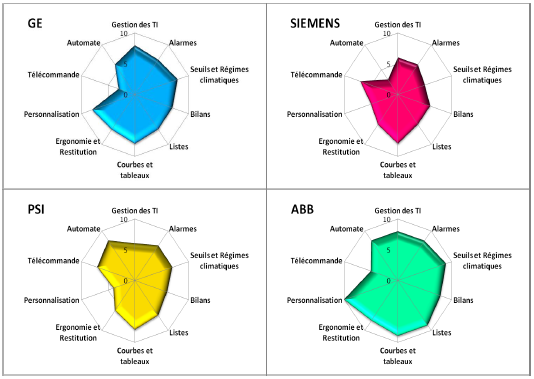
\includegraphics[width=0.7\textwidth]{0.figuras/Stanway_Kiviat_diagram_suppliers.png}}
    \captionof{figure}{Kiviat diagram of STANWAY suppliers. A detailed study was pursued for assessing project viability.}
    \label{fig:Kiviat_StanWay_supp}}
\end{figure}

StanWay expects to be a disruptive model of Rte's model information transfer system. Enclosed in an ancient automatons protocol system, Rte is in current transformation change of its TC network. StanWay will furnish a gateway between the users (SRC and SNC) and the clients, that is, the households and all the technology linked until them (see \autoref{fig:Kiviat_StanWay_users}).

\begin{figure}[h!]
    \centering
    \parbox[t]{0.7\textwidth}{
    \href{}{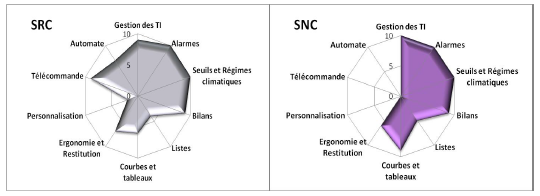
\includegraphics[width=0.7\textwidth]{0.figuras/Stanway_Kiviat_diagram_users.png}}
    \captionof{figure}{Kiviat diagram of STANWAY users. SRC and SNC are the highest level of automatons communications protocols at present.}
    \label{fig:Kiviat_StanWay_users}}
\end{figure}

\subsubsubsection{Apogee}
\label{sec:approach:project-approach:parties:apogee}

Tomorrow, driving systems must respond to an flexibilization and clients foreshight need. Apogeee seeks to redress this issue, and evolve the driving model towards a real-time managmenet navigation system, rather than an annual one. Apogee dispose several features for managing periodic maneuvers, parades, logging, reduction of losses or optimization of the network voltage plan, which will be subsequently taken over by Stanway.

\begin{figure}[h]
    \centering
    \parbox[t]{0.6\textwidth}{
    \href{http://collab.rte-france.com/SITES/cca/ref_architecture/AtRte/Pages/Accueil.aspx}{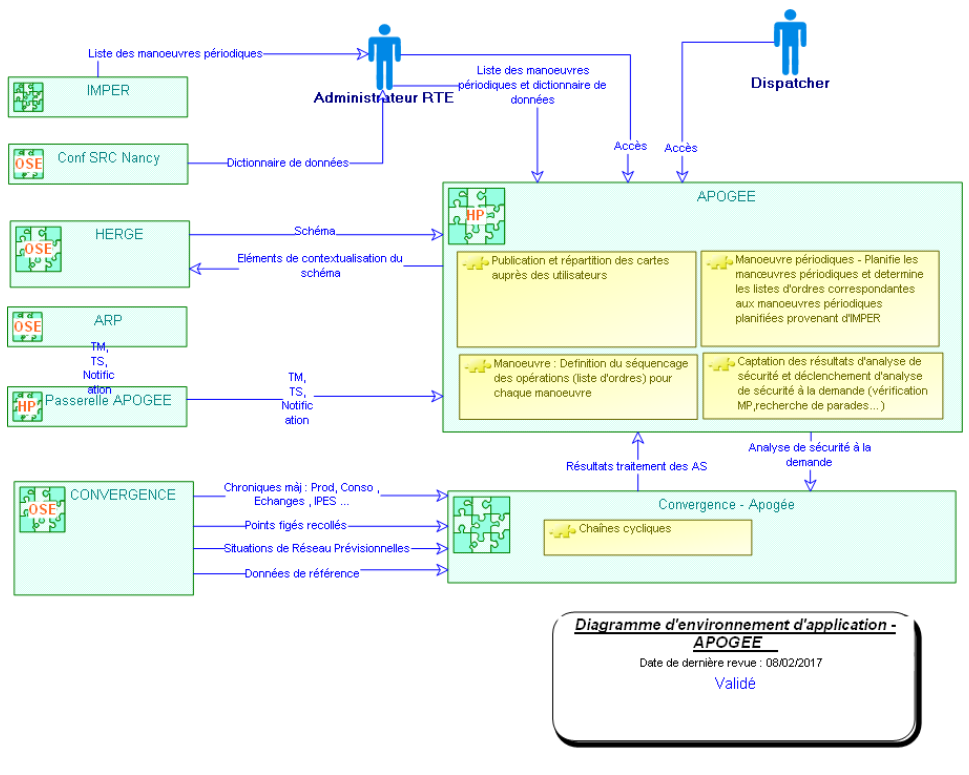
\includegraphics[width=0.6\textwidth]{0.figuras/diagram_APOGEE.png}}
    \captionof{figure}{Relational diagram between APOGEE \& HERGE. Click on the image to acces RTE's acronym database.}}
    \label{fig:APOGEE_diag}
\end{figure}

With a Java-software oriented approach\footnote{As most of the projects in the matter, Apogee was developed in Javascript. This providing feature performance advantages, their compatibility and flexibility remains notably inferior to FME's.}, Apogee opted for a much more user ergonomic canvass, where organs position may be modified to the user's taste after a primal page layout.

\begin{figure}[h]
    \centering
    \parbox[t]{0.45\textwidth}{
    \href{}{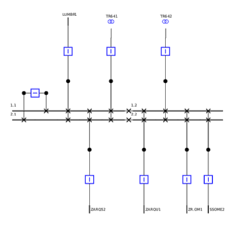
\includegraphics[width=0.45\textwidth]{0.figuras/TFM-Apogee-GAI.png}}
    \captionof{figure}{Prototype running in Apogee at Convergence.}}
    \label{fig:TFM-Apogee-GAI}
\end{figure}

\subsubsection{Risk assessement}
\label{subsub:introduction:thesis-purpose:risk-assessement}
On keeping with the aforementioned maxim, an additional difficulty pop up: notably, evaluating the impacts that the abovepresented concerned parties and others could have on the project's future. In this sense, several technical issues have been accordingly identified throughout the complete project, whom could be systematically approached and dealt with. Thus, a well-focused approach beforehand has decreased their impact and let to identify most of their consequences in advance.

Incertitude being well spread among different \nameref{subsub:introduction:thesis-purpose:project-approach:parties} on the modularity and adaptability have been the main maxima throughout the whole project, as result of a consequent risk assessment performed beforehand to the project.

As a result of this acknowledgement, \hyperref[fig:risk-matrix]{the following risk assessement matrix} charts the different inputs likely to impact the project, with an associated marginal weight on the project future scope: 

\begin{figure}[h!]
    \centering
    \parbox[t]{0.75\textwidth}{
    \href{}{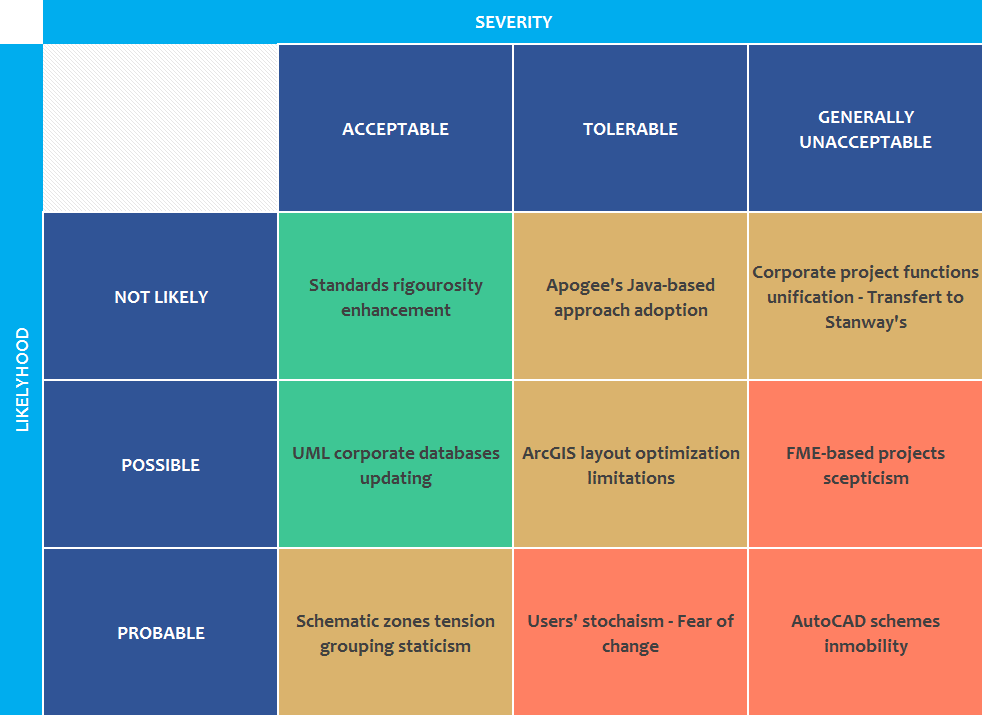
\includegraphics[width=0.75\textwidth]{0.figuras/risk-matrix.png}}
    \captionof{figure}{Hege risk matrix assessement.}
    \label{fig:risk-matrix}}
\end{figure}



% ---------------------------------------------------------------------

\subsection{Aim, scope and expected outcomes}
\label{sec:Intro:Thesis-purpose:Outcomes}
%REFORMULAR Y COMPLETAR

Digitalization is the order of the day in industrialization matters, although 15

On this pursuit, this project final aims to provide RTE with a comprehensible interface that could be extensible to multiple departments linked to SRC and SNC, and eventually enriched by the activities of STANWAY, APOGEE, ITESLA and other corporate projects embarked on the exploitation - real time management branch.
As sector trades are in continuous change in the last decade, tools digitization and data management is a constant in the matter and big companies as RTE must catch up the emerging technologies. Through all our contributions, we have intended to make the comings' work easier by providing them with a flexible and easily understandable network layout representation.  

Throughout all this document, it must remain clear to the reader what an important task lays on the rigorous and clear representation of the network. It will support most of the activities at ground level, where interdepartmental misunderstanding erupts as one of the major causes of fatal accidents in the sector. The latter delays the process development as all parts must be well concerned of any change and, therefore, corporate exemplars has to imperatively remain up to date. On top of that, numerous bureaucratic stages are internally stood so as to prevent for any error to take place \footnote{All them enriched simultaneously by the telecommute and telecontrol structure providing real time data of the network situation.}.

% ---------------------------------------------------------------------

% ---------------------------------------------------------------------
